% DONE CHAPTER!
\chapter{Sound and Hearing}

% DONE
\section{The Nature of Sound}
\paragraph{}A sound source, such as clapping two hands together in the air, causes the displacement of air particles.  The displacement of air particles at such a location forces the displaced particles closer to other air particles (condensation), resulting in an increase in the density of air.  There is then a reactive force, analogous to releasing a compressed spring, which causes the air particles to bounce away from each other (rarefaction), resulting in a decrease in the density of air at that location.  Sound waves propagate through a medium such as air, or water, through repeated condensation and rarefaction, and can be understood as a series of rapid changes in the density of a medium.

Sound is often analyzed in terms of amplitude and frequency.  Amplitude is the magnitude of vibration of a sound source (how much air is displaced), measured in decibels (dB), and frequency is the rate of vibration of a sound source (how often the air is displaced), measured in Hertz (Hz).  The perceptual correlates of amplitude and frequency are loudness, and pitch, respectively.  The frequency range of human hearing for young adults is 20-20000 Hz, and the sensitivity for high frequencies generally reduces as a natural progression of aging, known as age-related hearing loss, or presbycusis, which is the most common cause of hearing loss.

Sound is an important subject of study, because it helps us extract useful information from our environments.  Sound can warn us of potential dangers in our environments (e.g. fire alarms, traffic noise around a street corner, the growl of a predator in the jungle), as well as signal potential rewards (e.g. a prey's movements in a forest, the voice of a potential mate).  Most obviously, sound is a useful tool for communication through the mode of speech.  It is not surprising that, with hearing loss, it becomes more difficult to communicate with others, but it may surprise some to learn that hearing loss may often lead to social isolation \cite{Weinstein1982}, an increased probability of depression and anxiety \cite{Tambs2004}, and an increased risk of dementia \cite{Lin2011}.

Furthermore, speech is not the only mode of communication that relies on sound; there is also music.  Participating in musical activity has all sorts of demonstrated benefits; it has been shown to facilitate group trust and cooperation \cite{Anshel2004}, to be associated with greater cognitive abilities \cite{Schellenberg2004}, to prevent stress-induced anxiety \cite{Knight2001}, and to regulate one's mood \cite{Saarikallio2007}.

% DONE
\section{The Peripheral Auditory System}
\paragraph{}The human auditory pathway can be schematized as a hierarchy of processing blocks, organized from lower to higher levels, with connections between the blocks.  The processing blocks which respond to sound input sooner are commonly referred to as lower level, and are where basic features of the sound, such as amplitude, and frequency, are encoded.  More complex features, such as timbre, the formation of auditory objects, and detecting an auditory change, are governed by higher level processes and are largely mediated by later processing blocks.  For the most part, this thesis concerns itself only with the lower level auditory structures, often called the auditory periphery.  The auditory periphery is defined as all of the auditory structures and connections peripheral to the auditory brainstem in the auditory pathway, which includes the ear and auditory nerve.  In this thesis, little discussion will be given to the higher auditory structures.

% DONE
\subsection{Outer and Middle Ear}
\paragraph{}The peripheral auditory system is divided into three regions: the outer ear, the middle ear, and the inner ear.  An illustration of all regions can be seen in Figure 1.1.  The auditory canal and pinna make up the outer ear system \cite{Moore2007}.  When sound is directed at the ear, it is first shaped by interactions with the head and outer ear, which is well described by a head-related transfer function (HRTF) \cite{Wiener1946}.  The HRTF describes how frequencies are amplified and attenuated for different orientations of incoming sound, due to the natural ear canal and pinna resonances.  Several measurements of transfer functions have been taken over the years, and some of these data can be seen in Figure 1.2 \cite{Mehrgardt1977}.  For the most part, all of the transfer function measurements show the same overall shape, in that frequencies from 2-6 kHz are amplified by the natural resonances of the pinna and ear canal, with an additional peak occurring around 10 kHz.  It should be noted that this frequency response is not only dependent on the direction of the incoming sound, but also the frequency.  Medium and high frequencies are especially modified by the head, torso, and pinna \cite{Moore2007}, and in fact, the variations in the spectrum of the sound due to this shaping can be used to localize sound.

\begin{figure}[htbp]
\begin{center}
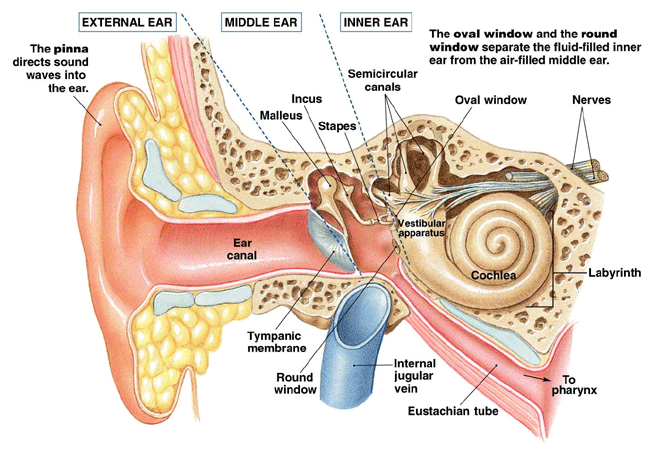
\includegraphics[height=3in]{chap1-hearing-and-balance.png} \\
\caption[Anatomy of the ear]{Anatomy of the ear.  The outer, middle, and inner ear and their components.  (Retrieved June 1, 2013, from: http://www.directhearingaids.co.uk/index.php/33/how-hearing-balance-work-together/)}
\label{ear-anatomy}
\end{center}
\end{figure}

\begin{figure}[htbp]
\begin{center}
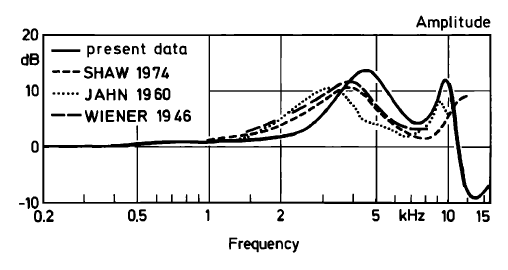
\includegraphics[height=3in]{chap1-outer-ear-transfer-function.png} \\
\caption[Outer ear transfer function]{Outer ear transfer function data obtained from different investigations.  A transfer function describes how different frequencies are amplified/attenuated as a result of traveling through the system.  (Reprinted from \citeA{Mehrgardt1977}).}
\label{outer-tf}
\end{center}
\end{figure}

Once sound has traveled down the auditory canal, it reaches the tympanic membrane, causing it to vibrate.  The tympanic membrane constitutes the beginning of the middle ear system.  Upon the tympanic membrane's vibration, it sets into motion a chain of three tiny bones (ossicles), named the incus, malleus, and stapes.  The stapes presses against the oval window of the cochlea, which has a surface area roughly 27 times smaller than the tympanic membrane \cite{Moore2007}, concentrating the acoustic energy into a smaller region through an impedance-matching process.  Impedance-matching in this context essentially means that the bones of the middle ear reduce the reflections off of the oval window that would otherwise occur if the sound transmission was through air, thereby maximizing the power transferred through the system.

Similar to the outer ear, the middle ear alters the frequency response of the incoming sound in a systematic fashion.  In particular, sounds between 500-5000 Hz are the most efficiently transmitted (see Figure 1.3), which is an important range for speech perception.  Also shown in Figure 1.3 is how the phase of the sound is altered by traveling through the middle ear system.  Notice how higher frequencies tend to be delayed longer than lower frequencies.

\begin{figure}[htbp]
\begin{center}
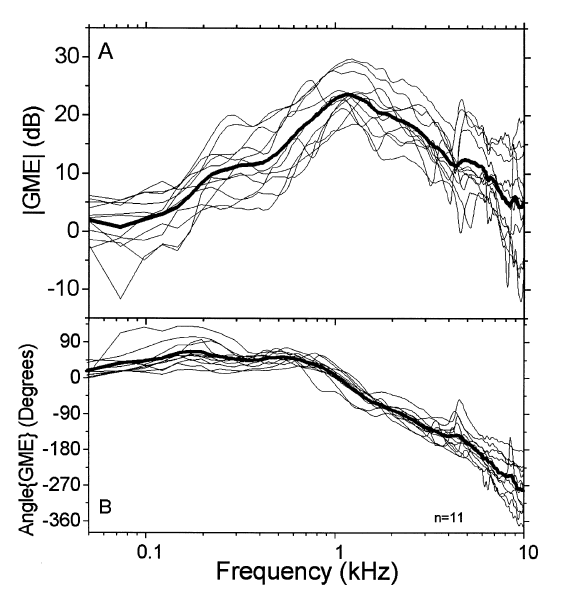
\includegraphics[width=3in]{chap1-middle-ear-transfer-function.png} \\
\caption[Middle ear transfer function]{Middle ear transfer function plotted for 11 ears (average in bold).  \emph{Top:} Magnitude response; the middle ear most efficiently transmits middle frequencies.  \emph{Bottom:} Phase response; higher frequencies are delayed more than lower frequencies.  (Reprinted from \citeA{Aibara2001}).}
\label{middle-tf}
\end{center}
\end{figure}

Thus far, both the outer and middle ear systems have been briefly described.  For the most part, both of these systems are linear; a linear system transforms an input abiding by two steadfast principles.  If an input to a linear system is scaled by a factor \emph{k}, the output must also be scaled by a factor \emph{k} (the scaling principle); and if two independent inputs, \emph{x} and \emph{y}, are presented to a linear system to produce separate outputs, \emph{o(x)} and \emph{o(y)}, then the response to \emph{x + y} summed together must equal \emph{o(x) + o(y)} (the superposition principle).  In the next section, the inner ear will be described, otherwise known as the cochlea, and in many cases we will observe that the cochlea behaves nonlinearly.

% DONE
\subsection{The Cochlea}
\paragraph{}The cochlea is a spiral shaped organ containing a series of fluid filled chambers, called the scala media, scala tympani, and scala vestibuli.  It begins with the oval window, which is the outermost shared boundary with the middle ear.  When the stapes of the middle ear presses upon the oval window, it causes the fluid in the scala vestibuli to flow to the scala tympani and eventually force the outward movement of another opening in the cochlea, called the round window.  The scala media is separated from the scala vestibuli by Reissner's membrane, and the scala media is separated from the scala tympani by the basilar membrane.  The movements of the oval window and the round window result in energy being absorbed by the basilar membrane, which causes it to vibrate, deflecting perpendicularly to its surface in the form of a traveling wave.  The traveling wave gradually grows in amplitude from the base of the cochlea to its maximal point of excitation (different for each frequency), at which point its amplitude quickly decreases.  The basilar membrane responds preferentially to different frequencies along its length, due to its elastic properties.  It is narrower and stiffer at the base, which high frequencies more easily resonate with, and it is wider at the apex, which lower frequencies preferentially resonate with (these physical properties are collectively referred to as the passive mechanism of the basilar membrane).  Thus, the basilar membrane is tonotopically arranged, encoding high frequencies at its base and low frequencies at its apex (see Figure 1.4), and each spot on the basilar membrane has a frequency it is most sensitive to, called a characteristic frequency (CF).  Another structure, called the tectorial membrane, forms a boundary with the basilar membrane, and between these two boundaries there are hair cells and nerve fibers which make up the organ of Corti (see Figure 1.5).

\begin{figure}[htbp]
\begin{center}
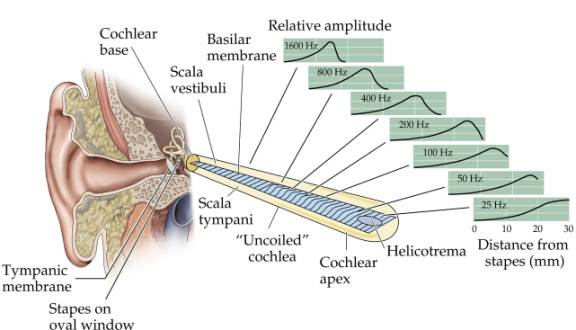
\includegraphics[width=4in]{chap1-uncoiled-cochlea.jpg} \\
\caption[The ``uncoiled" cochlea]{The ``uncoiled" cochlea.  The basilar membrane is tonotopically arranged; basal regions respond preferentially to high frequencies, and more apical regions respond preferentially to low frequencies.  (Retrieved June 1, 2013, from: http://www.rci.rutgers.edu/~uzwiak/AnatPhys/Audition.htm).}
\label{uncoiled-cochlea}
\end{center}
\end{figure}

% DONE
\subsubsection{Organ of Corti}

\begin{figure}[htbp]
\begin{center}
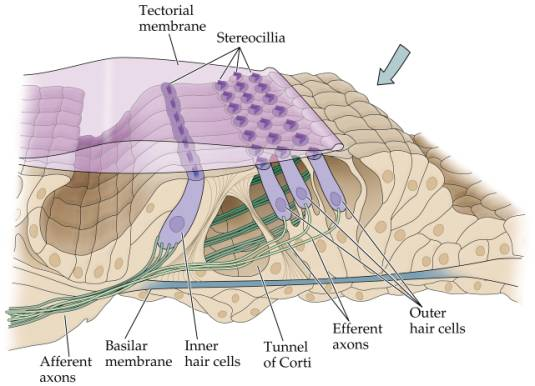
\includegraphics[width=4in]{chap1-organ-of-Corti.jpg} \\
\caption[Organ of Corti]{The organ of Corti holds the inner and outer hair cells and the auditory nerve fibers.  (Retrieved June 1, 2013, from:  http://www.rci.rutgers.edu/~uzwiak/AnatPhys/Audition.htm).}
\label{organ-of-Corti}
\end{center}
\end{figure}

\paragraph{}The organ of Corti rests upon the basilar membrane, inside the scala media.  It holds the outer hair cells (OHCs) and inner hair cells (IHCs), which are structurally different from one another and serve different functional purposes.  There are also nerve fibers which connect to these cells in the organ of Corti.  The nerve fibers are either afferent or efferent; the afferent nerve fibers primarily innervate the IHCs, and carry electrical impulses to higher auditory centres, while the efferent fibers' axons connect primarily to the OHCs.  Many of the efferent fibers originate from the superior olivary complex in the auditory brainstem.  The OHCs have a motor component and can change their length and stiffness, which actively shapes the basilar membrane response (this property is referred to as the active mechanism of the basilar membrane).  The tuning of the basilar membrane is thus a combination of a passive and active mechanism, and each mechanism alone cannot account for the basilar membrane's large vibration amplitude and narrow region of resonance \cite{Pickles2008}.

The OHCs are connected to the tectorial membrane, the other boundary of the organ of Corti, while the IHCs are not.  When the basilar membrane vibrates, it causes fluid motion in the scala media, while also causing the tectorial membrane to move back and forth in a shearing motion.  On the top of the OHCs and IHCs are tiny hairs called stereocilia, which are moved back and forth by the fluid motion in the scala media, or in the case of the OHCs, the shearing motion of the tectorial membrane.  When the basilar membrane deflects perpendicularly, the IHC stereocilia are moved back and forth, which results in a flow of electrical current through the cell, and the subsequent delivery of electrical impulses to the brain via the afferent nerve fibers described earlier.  Like the basilar membrane, each afferent nerve fiber has a CF, or a frequency for which it is most sensitive.

% DONE
\subsubsection{Nonlinear Cochlear Mechanics}
\paragraph{}In this section, the many nonlinearities of the cochlea will be described to provide a segue into how hearing aids have attempted to ameliorate the symptoms of hearing loss.

To begin, in a healthy ear, the basilar membrane behaves in a nonlinear manner, such that its amplitude of vibration grows nonlinearly with the intensity of the stimulus.  This is often referred to as the compressive nonlinearity of the basilar membrane, and can be illustrated with an input-output function (see Figure 1.6).  At low levels and very high levels, for a spot along the basilar membrane with a given CF, the input-output relation is near linear (a slope near 1), whereas for moderate levels, the input-output relation is compressive (a slope much less than 1).  Interestingly, when the stimulus frequency deviates from the CF, the input-output response becomes progressively more linear (see Figure 1.7).

\begin{figure}[htbp]
\begin{center}
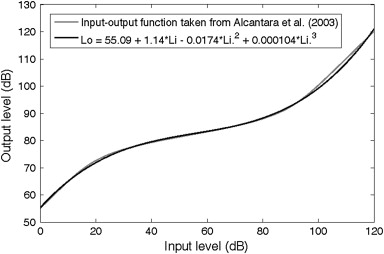
\includegraphics[width=3in]{chap1-basilar-membrane-nonlinearity.jpg} \\
\caption[Compressive nonlinearity of the basilar membrane]{Compressive nonlinearity of the basilar membrane.  For soft and loud sounds at a fixed place on the basilar membrane with a given CF, the input-output response is linear.  For moderate level sounds, the input-output response is compressive. (Reprinted from \citeA{Deroche2011}).}
\label{bm-compressive-nonlinearity}
\end{center}
\end{figure}

\begin{figure}[htbp]
\begin{center}
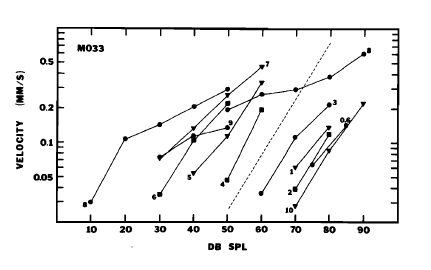
\includegraphics[width=3in]{chap1-basilar-membrane-nonCF.png} \\
\caption[Basilar membrane response with deviations from the CF]{Separate input-output curves plotted for several different frequencies.  All measurements were taken at the same place on the basilar membrane, which had a CF of 8 kHz.  The input-output response is progressively more linear for frequencies which deviate from the CF.  (Reprinted from \citeA{Robles1986}).}
\label{bm-nonCF}
\end{center}
\end{figure}

Another psychoacoustic phenomenon, called two-tone suppression, introduces a nonlinearity in the way the basilar membrane responds to complex sounds.  In essence, when two pure tones with different frequencies are presented simultaneously, one tone (the suppressor) may suppress the basilar membrane response to the other tone (the probe), particularly when the suppressor is greater in intensity (see Figure 1.8), and close to the probe tone frequency (see Figure 1.9).

\begin{figure}[htbp]
\begin{center}
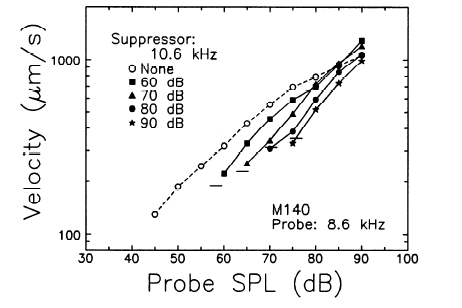
\includegraphics[width=3in]{chap1-two-tone-suppression.png} \\
\caption[Two-tone suppression - effects of intensity]{Basilar membrane amplitude velocity as a function of the probe tone level (in dB SPL).  When the level of the suppressor tone is increased, the level of the probe tone required to reach criterion velocity of the basilar membrane also increases.  (Reprinted from \citeA{Ruggero1992}).}
\label{two-tone-1}
\end{center}
\end{figure}

\begin{figure}[htbp]
\begin{center}
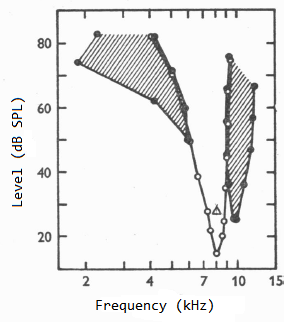
\includegraphics[width=3in]{chap1-two-tone-suppression-2.png} \\
\caption[Two-tone suppression - effects of frequency]{The effect of two-tone suppression on an individual tuning curve (white circles), for a neuron with a CF of 8 kHz.  The neuron was stimulated with the probe tone at a given intensity (indicated by the triangle), and a suppressor tone was varied in frequency and intensity.  Tones within the shaded region reduced the response of the probe tone by 20\%.  (Reprinted from \citeA{Arthur1971}).}
\label{two-tone-2}
\end{center}
\end{figure}

Similar to two-tone suppression, when two tones are presented simultaneously and their frequencies are not too far apart from each other, distortion products are generated at linear combinations of the two frequencies (2f1 - f2, f2 - f1, etc.).  These distortion products even behave like separate sinusoidal tones, causing vibration on the basilar membrane at locations with those CFs \cite{Moore2007}.

\begin{figure}[ht]
\begin{center}
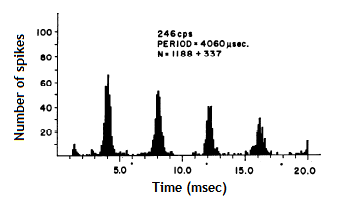
\includegraphics{chap1-phase-locking.png} \\
\caption[Phase locking]{An illustration of phase locking.  Auditory nerve fibers fire at a particular phase of the stimulus waveform.  For a tone with a frequency of approximately 250 Hz, and a corresponding period of 4 msec, the peak firing rate occurs every 4 msec.  (Adapted and reprinted from \citeA{Rose1967}).}
\label{phase-locking}
\end{center}
\end{figure}

One last nonlinear component to cochlear mechanics is the concept of phase locking.  When an AN fiber responds to a tone presented at its CF, it responds in a predictable way, firing at a particular phase in the waveform (see Figure 1.10).  Phase locking only occurs for sufficiently low frequency stimuli (less than 5 kHz, according to \cite{Pickles2008}); it is stimulus dependent, not AN dependent, meaning that an AN fiber with a high CF is able to phase lock to sufficiently low frequency stimuli.

\section{Hearing Loss}
\paragraph{}Hearing loss is widespread, affecting 11\% of the US population to some degree \cite{Kochkin2009}.  This proportion is likely to grow in the coming decade due to an aging population, increasing noise pollution \cite{Goines2007}, and the pervasive use of personal audio devices, which afford listeners the opportunity to expose themselves to potentially damaging sound levels on a more frequent basis.

Hearing loss is generally classified as either conductive, sensorineural (SNHL), or mixed, depending on the nature and location of the damage.  A conductive loss is defined as any problem in the conduction of sound waves from the outer to the inner ear, and can be caused by factors such as wax buildup, an accumulation of fluids, the degradation of the ossicles, or a perforated ear drum.  It is characterized by significantly higher air-conduction thresholds than bone-conduction thresholds.  Sensorineural impairments are localized in the inner ear, and are typified by the degradation of OHCs or IHCs or the malfunction of AN fibers in the inner ear.  This thesis only concerns itself with SNHL, the most prevalent form of hearing loss.

To quantify one's level of hearing loss, one generally visits a hearing clinic to have a hearing test administered by an audiologist or a hearing instrument specialist.  During the hearing test, the participant is seated in a sound booth wearing headphones, and the audiologist plays pure tones of different frequencies through the headphones, one by one, using an instrument called an audiometer.  Depending on the clinic's available equipment, the participant signals that they can hear a pure tone by pressing a button or by raising their hand.  The intensity of the pure tone is adaptively adjusted to find the threshold at which the listener can consistently hear the pure tone.  At the end of the test, using the data collected, the audiologist creates an audiogram, which quantifies the level of hearing loss in units of dB HL for the listener at specific frequencies, generally ranging from 250 Hz to 8000 Hz (see Figure 1.11).  dB HL stands for decibels Hearing Level, which is a standard used to define how many more decibels one requires over a normal, young listener, in order to hear a sound at a particular frequency.  The most common shape of hearing loss is a sloping hearing loss, such that the higher frequencies are more damaged than the lower frequencies.

\begin{figure}[htbp]
\begin{center}
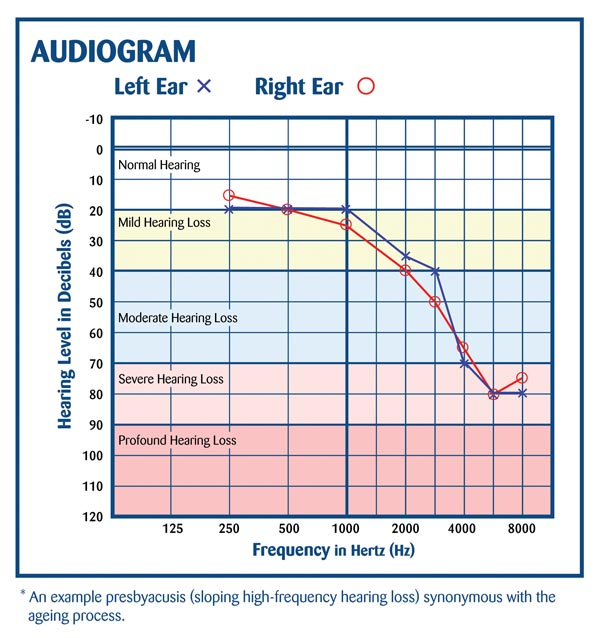
\includegraphics[width=3in]{chap1-audiogram-presbycusis.jpg} \\
\caption[Audiogram with presbycusis]{An audiogram with presbycusis, sloping from low to high frequency.  Hearing loss is graded from mild to severe on the dB HL scale, measured at specific frequencies ranging from 250 to 8000 Hz.  Both the left and right ears are plotted.  (Retrieved June 1, 2013, from: http://auditoryneuroscience.com/acoustics/clinical\_audiograms).}
\label{audiogram-schematic}
\end{center}
\end{figure}

With OHC loss, there is a loss of frequency sensitivity and selectivity, which can be observed as a greater threshold of activation for an individual AN fiber, and a broader tuning curve, respectively (see Figure 1.12).  The corresponding effect on perception is a loss of audibility and clarity, and sounds become especially susceptible to masking in noise.  Another way of illustrating the effect of the loss of OHCs is to observe that the input-output response of the basilar membrane shifts to the right and behaves more linearly (see Figure 1.13).

\begin{figure}[htbp]
\begin{center}
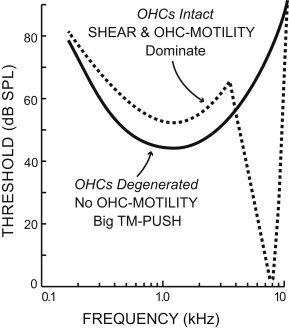
\includegraphics[width=2.5in]{chap1-OHCloss.jpg} \\
\caption[Stylized tuning curve with and without OHC loss.]{Stylized tuning curve with and without OHC loss.  When OHCs are intact, the tuning curve is very narrow.  Losing the OHCs broadens the tuning curve, and results in a loss of sensitivity due to the failing active mechanism which provides gain at low intensities.  (Reprinted from \citeA{Guinan2012}).}
\label{bm-OHCloss}
\end{center}
\end{figure}

\begin{figure}[htbp]
\begin{center}
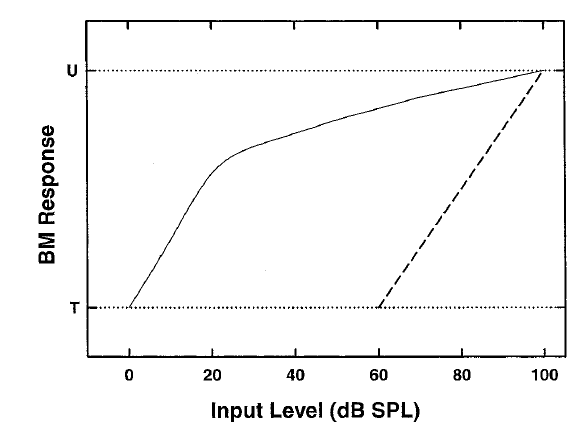
\includegraphics[width=2.5in]{chap1-basilar-membrane-linear-after-loss.png} \\
\caption[Linear basilar membrane response following OHC loss]{The basilar membrane response amplitude following OHC loss.  A healthy basilar membrane response exhibits nonlinearity (solid line), while loss of OHCs results in a more linear response (dashed line).  On the ordinate, T represents threshold and U represents uncomfortable loudness. (Reprinted from \citeA{Oxenham2003}).}
\label{bm-after-loss}
\end{center}
\end{figure}

IHC loss, contrary to OHC loss, does not affect the compressive nonlinearity of the basilar membrane, as is indicated by a normal cochlear microphonic (CM) and intact distortion product otoacoustic emissions (DPOAEs) \cite{Trautwein1996}.  IHC loss also does not significantly affect the threshold and tuning of remaining AN fibers \cite{Wang1997}.  However, loss of IHCs does reduce the output of the cochlea, as measured by a reduction in the amplitude of the compound action potential (CAP) \cite{Trautwein1996, Qiu2000}.  Interestingly, in the Qiu et al. paper, despite a reduced amplitude for the CAP and inferior colliculus potential (ICP), some animals showed an increase in the auditory cortex potential (ACP) amplitude, reflecting an increased gain in the central auditory system.  In fact, the increased gain in the central auditory system has been proposed as a compensatory mechanism for reduced input from the cochlea, and could be the mechanism driving the perception of tinnitus \cite{Norena2011}, which is often described as a phantom ringing or hissing sensation.  Recent evidence from chinchillas has shown that significant loss of IHCs results in very minor audiometric threshold shifts, and therefore audiograms may not provide much information about IHC loss \cite{Lobarinas2013}.

Temporal coding in the cochlea is altered with SNHL as a result of the broadened frequency tuning curves observed for AN fibers.  Two ways of measuring temporal properties of an AN fiber is to look at its phase response and its group delay.  The phase response describes how the signal is delayed as a function of frequency, and group delay is the total length of time it takes for the signal to be processed by the auditory filter.  With a broadened tuning curve, the phase response becomes shallower (see Figure 1.14), and there is a shorter group delay \cite{Shi2006}.  Also, there is psychophysical evidence suggesting that SNHL affects one's ability to use temporal fine-structure cues for speech perception \cite{Lorenzi2006, Hopkins2008}, which is not entirely surprising, given that the temporal coding properties of individual AN fibers are altered with SNHL.

\begin{figure}[htbp]
\begin{center}
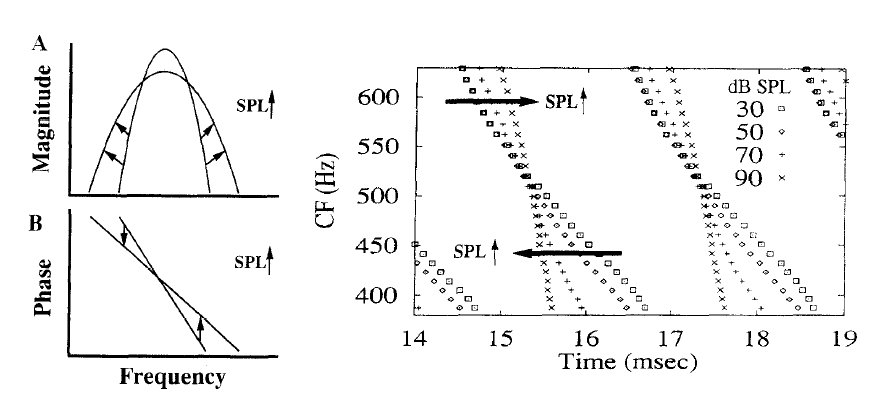
\includegraphics[width=\textwidth]{chap1-phase-response-concatenated.png} \\
\caption[AN magnitude and phase response with increasing stimulus level]{\emph{A:} with increasing stimulus level, an AN fiber's tuning curve broadens, similar to what happens with OHC loss.  \emph{B:} with increasing stimulus level, the slope of the phase response of an AN fiber becomes shallower.  \emph{Right:} with increasing stimulus level, the group delay decreases. (Reprinted from \citeA{Carney1994}).}
\label{phase-response}
\end{center}
\end{figure}

As mentioned in the previous section, phase locking is an important nonlinearity of a healthy ear.  In ears with SNHL, however, the tuning curves of AN fibers are shifted toward lower CFs and become broader.  The result is that these shifted AN fibers begin to phase lock and synchronize to lower frequency stimuli, which is called an upward spread of synchrony \cite{Miller1997}.  This presents a problem for speech perception, since the formants are very important for speech intelligibility \cite{Peterson1952, Kiefte2010}; higher formants may not be properly encoded in ears with SNHL, which could result in confusability between the formants, and therefore reduced speech intelligibility.

In summary, SNHL is a pervasive disorder and can be caused by dysfunction of any of the following: IHCs, OHCs, or AN fibers.   With SNHL, the response properties of individual AN fibers are altered in numerous ways, disrupting the neural code at the level of the AN.  Disruptions in the neural code may degrade speech intelligibility, which is a common complaint of those with SNHL, especially in the presence of background noise.  Other auditory abilities, such as music perception and sound localization, may be similarly affected by a disrupted neural code in the auditory nerve.  The purpose of this thesis is to compare two hearing aid algorithms on their efficacy of restoring these auditory abilities; one algorithm proposes to restore a neural code closer to normal, and the other algorithm is a standard prescription in the hearing aid industry.  The next chapter introduces these hearing aid algorithms, among other hearing aid components and features, in more detail. 